\newpage
\section{Mô hình hồi quy tuyến tính đa thức}

\paragraph{}{\textbf{Hồi quy tuyến tính đa thức} \cite{ostertagova2012modelling} (Polynomial regression) là một dạng hồi quy mở rộng của hồi quy tuyến tính, trong đó mối quan hệ giữa biến độc lập và biến phụ thuộc không phải là một đường thẳng mà là một đa thức bậc cao hơn. Ngoài ra, hồi quy tuyến tính đa thức còn là mô hình hiệu quả để đánh giá các mối quan hệ phi tuyến tính giữa các giá trị đầu vào và đầu ra, đặc biệt hữu dụng khi phân loại các dữ liệu cần đường hồi quy phức tạp.}

\paragraph{}{Với hồi quy tuyến tính đa thức, mô hình được mở rộng thành các bậc cao hơn của biến độc lập X. Mô hình hồi quy đa thức đơn biến bậc n có dạng:}

\begin{center}
\large $Y = \beta_0+\beta_1*X+\beta_2*X^2+...+\beta_k*X^k + \epsilon$
\end{center}

Trong đó:
\begin{itemize}
    \item $k$: Bậc của đa thức
    \item $X$: Biến độc lập
    \item $Y$: Biến phụ thuộc
    \item $\epsilon$: Thành phần sai số
    \item $\beta_0$: Hệ số chặn (intercept)
    \item $\beta_1,\beta_2...,\beta_k$: Các hệ số hồi quy (coefficient)
\end{itemize}

\subsection{Xây dựng mô hình}
\subsubsection{Phương pháp xây dựng}

\paragraph{}{Nếu coi mỗi lũy thừa của biến độc lập như một biến độc lập mới: $X_1 = X, X_2 = X^2, X_3 = X^3, ...$. Ta nhận thấy rằng mô hình hồi quy đa thức trở thành:}

\begin{center}
\large $Y = \beta_0+\beta_1*X_1+\beta_2*X_2+...+\beta_k*X_k + \epsilon$
\end{center}

\paragraph{}{Nhận xét: Qua mô hình trên thấy được hồi quy tuyến tính đa thức là một dạng đặc biệt của hồi quy tuyến tính đa biến (Multiple Linear Regression) (xem ở \ref{label:lr}). Vì vậy để xây dựng mô hình hồi quy tuyến tính đa thức, ta có thể xây dựng dựa vào mô hình hồi quy đa biến với các đặc trưng đa thức $[X, X^1, X^2,X^3,...,X^k]$.}

\paragraph{}{Ta sử dụng \textbf{phương pháp bình phương tối thiểu} (Ordinary Least Squares - OLS) (xem \ref{label:simple-linear}) hoặc \textbf{phương pháp Gradient Descent} (xem \ref{label:GradientDecent}) để giải quyết bài toán. Ngoài ra, ta có thể sử dụng thêm kỹ thuật \textbf{Chính quy hóa} (Regularization) với L1 (Lasso) (xem \ref{label:lasso-math}) hoặc L2 (Ridge) (xem \ref{label:ridge-math}) để giảm tình trạng overfitting hoặc giải được bài toán hồi quy đa thức bậc cao với nhiều đặc trưng (đa biến) có bao gồm sự tương tác giữa các đặc trưng với nhau.}

\subsubsection{Xây dựng đặc trưng đa thức}
\paragraph{a) Giới thiệu:}{Đặc trưng đa thức là các đặc trưng mới được xây dựng từ các đặc trưng đầu vào gốc bằng cách nâng bậc chúng lên. Ví dụ:}
\paragraph{}{Với một biến đầu vào x:}
\begin{itemize}
    \item Bậc 1: $x$ (đặc trưng gốc)
    \item Bậc 2: $x, x^2$
    \item Bậc 3: $x, x^2, x^3$
    \item ...
    \item Bậc k: $x, x^2, x^3, ..., x^k$
\end{itemize}
\paragraph{}{Với hai biến đầu vào $x_1$ và $x_2$ (Bao gồm sự tương tác giữa các biến):}
\begin{itemize}
    \item Bậc 1: $x_1, x_2$ (đặc trưng gốc)
    \item Bậc 2: $x_1, x_2, x_1^2, x_2^2, x_1*x_2$
    \item Bậc 3: $x_1, x_2, x_1^2, x_2^2, x_1*x_2, x_1^3, x_2^3, x_1^2*x_2, x_1*x_2^2$
    \item ...
\end{itemize}
\paragraph{}{Tương tự với các trường hợp biến đầu vào nhiều hơn 2. Vì vậy sau khi áp dụng biến đổi đa thức với bậc d, chúng ta sẽ thu được ma trận đặc trưng đa thức $X_{poly}$ với kích thước $n*m$, trong đó m là số lượng đặc trưng đa thức được tạo ra tính bằng công thức dưới.}

\paragraph{b) Công thức tính tổng quát số lượng đặc trưng đa thức:}{}
\begin{center}
\large $C(k + d, d) = \binom{k + d}{d} = \frac{(k + d)!}{d! * k!}$
\end{center}
Trong đó:
\begin{itemize}
    \item $C(k + d, d)$: tổ hợp chập $d$ của $k + d$.
    \item $k$: số lượng biến đầu vào (features) ban đầu.
    \item $d$: bậc đa thức tối đa.
\end{itemize}

\paragraph{c) Ma trận hóa:}{Quá trình ma trận hóa đặc trưng đa thức thực hiện biến đổi trên từng hàng (mẫu) của ma trận đầu vào $\mathbf{X}$ để tạo ra một hàng mới trong ma trận $\mathbf{X_{poly}}$.}

\paragraph{}{Ví dụ minh họa với 2 biến đầu vào (k=2) và bậc đa thức d=2:}

\paragraph{}{Giả sử chúng ta có một mẫu dữ liệu duy nhất $\mathbf{x} = \begin{pmatrix} x_1 & x_2 \end{pmatrix}$ và chúng ta muốn tạo đặc trưng đa thức bậc 2. Các đặc trưng đa thức được tạo ra là:}

\begin{enumerate}
    \item Bậc 0: $1$ (bias term)
    \item Bậc 1: $x_1, x_2$
    \item Bậc 2: $x_1^2, x_1x_2, x_2^2$
\end{enumerate}

\paragraph{}{Như vậy, vector đặc trưng đa thức cho mẫu $\mathbf{x}$ sẽ là:}

$$
\mathbf{x_{poly}} = \begin{pmatrix} 1 & x_1 & x_2 & x_1^2 & x_1x_2 & x_2^2 \end{pmatrix}
$$

\paragraph{}{Tổng quát hóa cho ma trận X:}

\paragraph{}{Để tạo ma trận $\mathbf{X_{poly}}$ từ ma trận $\mathbf{X}$, chúng ta sẽ áp dụng biến đổi trên cho từng hàng của $\mathbf{X}$.\newline

Ví dụ, nếu ma trận đầu vào $\mathbf{X}$ là:}

$$
\mathbf{X} =
\begin{pmatrix}
  x_{11} & x_{12} \\
  x_{21} & x_{22} \\
  x_{31} & x_{32}
\end{pmatrix}
$$

\paragraph{}{Thì ma trận đặc trưng đa thức $\mathbf{X_{poly}}$ bậc 2 sẽ là:}

$$
\mathbf{X_{poly}} =
\begin{pmatrix}
  1 & x_{11} & x_{12} & x_{11}^2 & x_{11}x_{12} & x_{12}^2 \\
  1 & x_{21} & x_{22} & x_{21}^2 & x_{21}x_{22} & x_{22}^2 \\
  1 & x_{31} & x_{32} & x_{31}^2 & x_{31}x_{32} & x_{32}^2
\end{pmatrix}
$$

\paragraph{}{Dựa trên ma trận hóa của mô hình \textbf{hồi quy đa biến (Multiple Regression)} (xem \ref{label:simple-linear}). Đối với toàn tập dữ liệu có $n$ quan sát và $m$ đặc trưng đa thức (features), ta có thể biểu diễn tổng quát ma trận hồi quy:}

\begin{equation}
    \begin{bmatrix}
        y_1 \\
        y_2 \\
        \vdots \\
        y_n
    \end{bmatrix}
    _{\text{$n \times 1$}}
    = 
    \begin{bmatrix}
        1 & x_{11} & x_{12} & \dots & x_{11}^2 & x_{12}^2 & \dots & x_{11} \cdot x_{12} & \dots\\
        1 & x_{21} & x_{22} & \dots & x_{21}^2 & x_{22}^2 & \dots & x_{21} \cdot x_{22} & \dots \\
        \vdots & \vdots & \vdots & \ddots & \vdots & \vdots & \ddots & \vdots & \ddots \\
        1 & x_{n1} & x_{n2} & \dots & x_{n1}^2 & x_{n2}^2 & \dots & x_{n1} \cdot x_{n2} & \dots \\
    \end{bmatrix}
    _{\text{$n \times m$}}
    \begin{bmatrix}
        \beta{0} \\
        \beta{1} \\
        \vdots \\
        \beta{m}
    \end{bmatrix}
    _{\text{$m \times 1$}}
    +
    \begin{bmatrix}
        \epsilon_{1} \\
        \epsilon_{2} \\
        \vdots \\
        \epsilon_{n}
    \end{bmatrix}
    _{\text{$n \times 1$}}
\end{equation}

\paragraph{}{Phương trình này có thể được biểu diễn một cách ngắn gọn hơn trong ký hiệu ma trận:}

\begin{equation}
    \mathbf{Y} = \mathbf{X_{poly}}\boldsymbol{\beta} + \epsilon
\end{equation}

Trong đó:
\begin{itemize}
    \item $\mathbf{Y} \in \mathbb{R}^{n \times 1}$ là vector cột chứa $n$ giá trị phụ thuộc
    \item $\mathbf{X} \in \mathbb{R}^{n \times m}$ là ma trận chứa $n$ mẫu quan sát với $m$ đặc trưng đa thức cho mỗi mẫu
    \item $\boldsymbol{\beta} \in \mathbb{R}^{m \times 1}$ là vector hệ số hồi quy cần ước lượng
    \item $\epsilon \in \mathbb{R}^{n \times 1}$ là giá trị thành phần sai số ngẫu nhiên (the random error component)
\end{itemize}

\paragraph{d) Nhận xét:}{Bậc của đa thức là một hyperparameter quan trọng trong hồi quy đa thức. Việc lựa chọn bậc phù hợp có ảnh hưởng lớn đến hiệu suất của mô hình:}
\begin{itemize}
    \item Bậc quá thấp (Underfitting): Mô hình quá đơn giản, không thể nắm bắt được các mẫu phức tạp trong dữ liệu. Dẫn đến sai số cao trên cả dữ liệu huấn luyện và dữ liệu kiểm tra.

    \item Bậc vừa phải (Good Fit): Mô hình có độ phức tạp vừa đủ để nắm bắt được các mẫu quan trọng trong dữ liệu mà không quá khớp. Đạt được hiệu suất tốt trên cả dữ liệu huấn luyện và dữ liệu kiểm tra.

    \item Bậc quá cao (Overfitting): Mô hình quá phức tạp, khớp quá sát với dữ liệu huấn luyện, bao gồm cả nhiễu. Dẫn đến sai số thấp trên dữ liệu huấn luyện nhưng sai số cao trên dữ liệu kiểm tra (khả năng tổng quát hóa kém).
\end{itemize}

\subsubsection{Huấn luyện mô hình}
\paragraph{}{Để huấn luyện mô hình \textbf{hồi quy đa thức (Polynomial Regression)} ta có thể sử dụng quá trình huấn luyện mô hình bằng phương pháp Gradient Descent của \textbf{hồi quy đa biến (Multiple Regression)} (xem \ref{label:GradientDecent}) dựa trên đặc trưng đa thức được xây dựng ở trên.}

\paragraph{}{\textbf{Các tham số:}}
\begin{itemize}
    \item Learning rate: 0.01
    \item Số epoch: 5000
    \item Batch size: 32
    \item Epsilon: $10^{-8}$ (Ngưỡng hội tụ)
\end{itemize}

\paragraph{}{\textbf{Triển khai:}}
\begin{itemize}
    \item Dữ liệu huấn luyện được sắp xếp ngẫu nhiên trước mỗi epoch để giảm thiểu phương sai trong quá trình cập nhật trọng số.
    \item Batch Gradient Descent được sử dụng để cập nhật trọng số mô hình.
    \item Lưu lại bộ trọng số tốt nhất trong quá trình huấn luyện.
\end{itemize}

\paragraph{}{\textbf{Quá trình huấn luyện:}}

\begin{figure}[H]
    \centering
    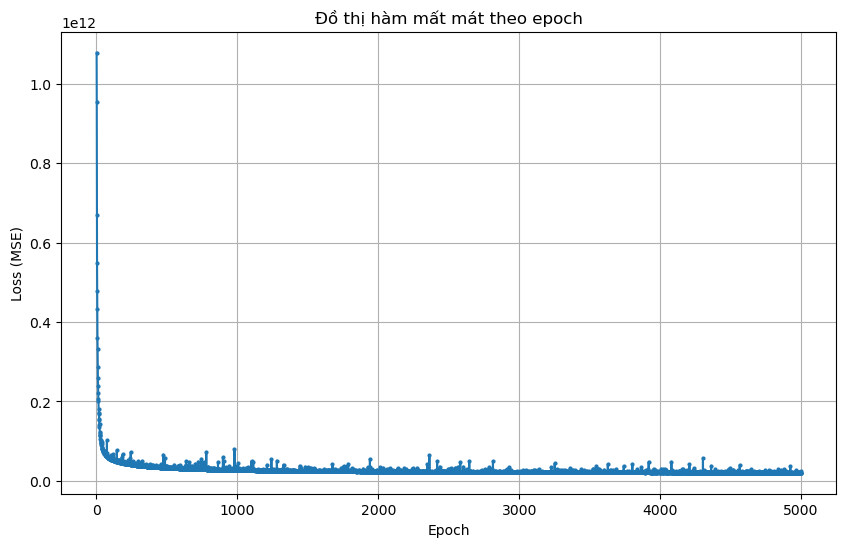
\includegraphics[width=0.7\textwidth]{img/Poly_Loss_Plot.png}
    \caption{Biểu đồ Loss qua các Epoch.}
    \label{fig:poly-loss_plot}
\end{figure}

\begin{itemize}
    \item Biểu đồ cho thấy giá trị hàm mất mát (Loss) giảm dần theo số epoch, chứng tỏ mô hình đang học được các mẫu từ dữ liệu huấn luyện.
    \item Ban đầu, loss rất lớn (khoảng hơn $10^{12}$), nhưng sau 5000 epoch, nó giảm xuống đáng kể còn khoảng $2 * 10^{10}$.
    \item Mô hình đạt được giá trị loss tối ưu (trên tập huấn luyện là $20342161463.87$)
\end{itemize}

\subsubsection{Công thức hồi quy}
\paragraph{}{Hiển thị top 10 số hạng dựa trên hệ số hồi quy lớn nhất:}

\begin{center}
\small $Price = 1680790.7703 \cdot Model + 1559994.1677 \cdot Model \cdot Year + 1464639.3648 \cdot Model \cdot Year^2 + 1046459.7736 \cdot Model \cdot Transmission + 1046459.7736 \cdot Model \cdot Transmission^2 + 1009863.5419 \cdot Model \cdot Kilometer + 946888.0919 \cdot Model \cdot Year \cdot Transmission + 938621.1008 \cdot Model \cdot Location + 938621.1008 \cdot Model \cdot Location^2 + 935093.6800 \cdot Model \cdot Year \cdot Kilometer + ...$
\end{center}

Trong đó:
\begin{itemize}
    \item $Price$: Giá xe được dự đoán bởi mô hình
    \item $Model, Year, Transmission, ...$: Giá trị của các đặc trưng trong tập dữ liệu sau các quá trình xử lí dữ liệu.
\end{itemize}

Nhận xét: Dựa vào công thức hồi quy, ta thấy \texttt{Model} là đặc trưng tốt nhất có khả năng tương quan thuận với \texttt{Price}. Ngoài ra, các đặc trưng như \texttt{Year}, \texttt{Tranmission} cũng có sự ảnh hưởng lớn đến giá trị \texttt{Price}.

\subsection{Đánh giá mô hình}

\begin{figure}[H]
    \centering
    \begin{subfigure}[b]{0.48\textwidth}
        \centering
        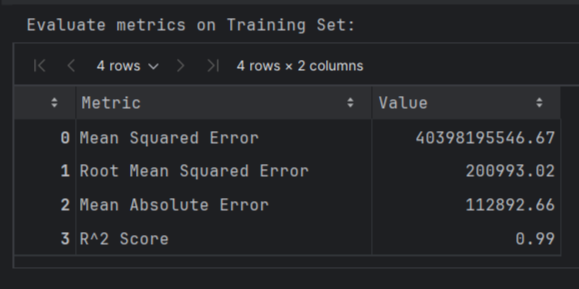
\includegraphics[width=\linewidth]{img/Evaluate_Poly_Training_Set.png}
        \caption{Đánh giá trên tập huấn luyện}
        \label{fig:poly-linear-train}
    \end{subfigure}
    \hfill
    \begin{subfigure}[b]{0.48\textwidth}
        \centering
        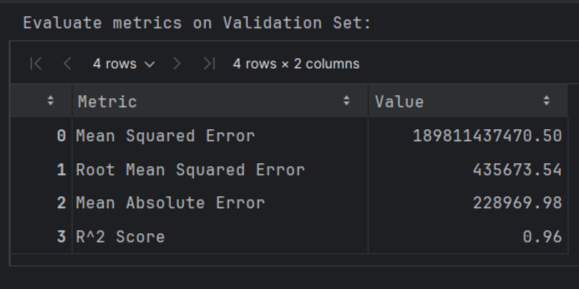
\includegraphics[width=\linewidth]{img/Evaluate_Poly_Validation_Set.png}
        \caption{Đánh giá trên tập kiểm chứng}
        \label{fig:poly-linear-valid}
    \end{subfigure}
    \caption{So sánh đánh giá mô hình hồi quy đa thức bậc 3 trên tập huấn luyện và kiểm chứng} 
    \label{fig:poly-linear-eval}
\end{figure}

\paragraph{}{Trên tập huấn luyện, mô hình đạt MSE là $40398195546.67 \approx 4.0398 * 10^{10}$ và R² là $0.99$, cho thấy mô hình rất khớp với dữ liệu đã thấy. Tuy nhiên, trên tập kiểm chứng, MSE tăng lên đáng kể thành $189811437470.50 \approx 1.8981 * 10^{11}$ và R² giảm xuống còn $0.96$.}

\paragraph{}{Mặc dù giá trị R² trên tập kiểm chứng vẫn khá cao, sự gia tăng đáng kể của các chỉ số lỗi (MSE tăng gấp $5$ lần, RMSE và MAE tăng gấp $2$ lần) cho thấy dấu hiệu của hiện tượng overfitting. Mô hình đã học thuộc một số đặc điểm nhiễu của tập huấn luyện và khả năng tổng quát hóa trên dữ liệu mới bị hạn chế hơn. Điều này cũng có thể quan sát thấy trong hình \ref{fig:poly-linear-eval}, nơi các điểm dữ liệu kiểm chứng phân tán rộng hơn quanh đường dự đoán so với tập huấn luyện.}

\begin{figure}[H]
    \centering
    \begin{subfigure}[b]{1\textwidth} % Tăng chiều rộng lên để ảnh chiếm gần hết chiều rộng trang
        \centering
        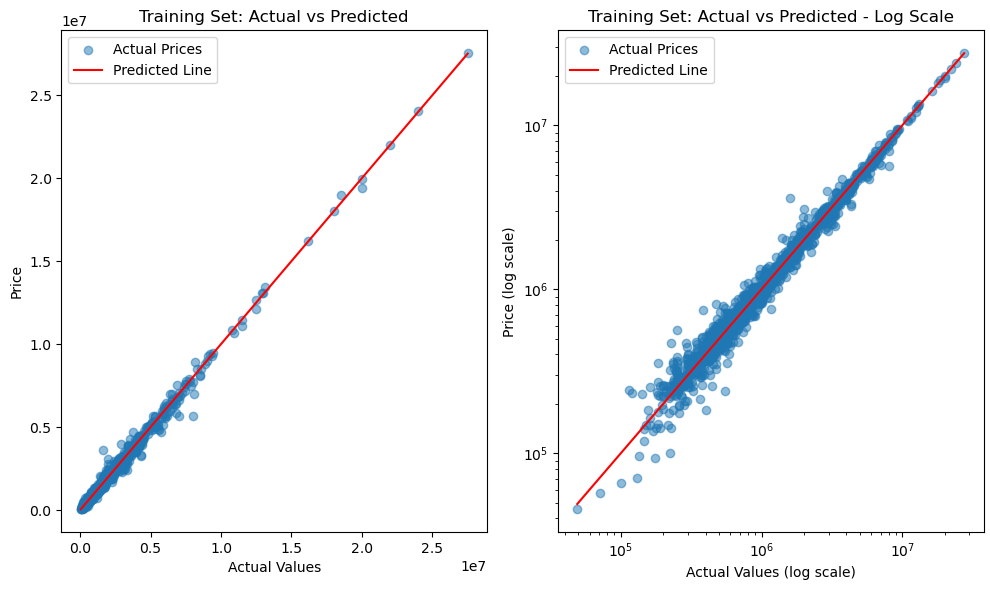
\includegraphics[width=\linewidth]{img/Poly_Training_Plot.png}
        \caption{Đánh giá trên tập huấn luyện}
        \label{fig:poly-linear-train-plot}
    \end{subfigure}

    \begin{subfigure}[b]{1\textwidth} % Tăng chiều rộng lên để ảnh chiếm gần hết chiều rộng trang
        \centering
        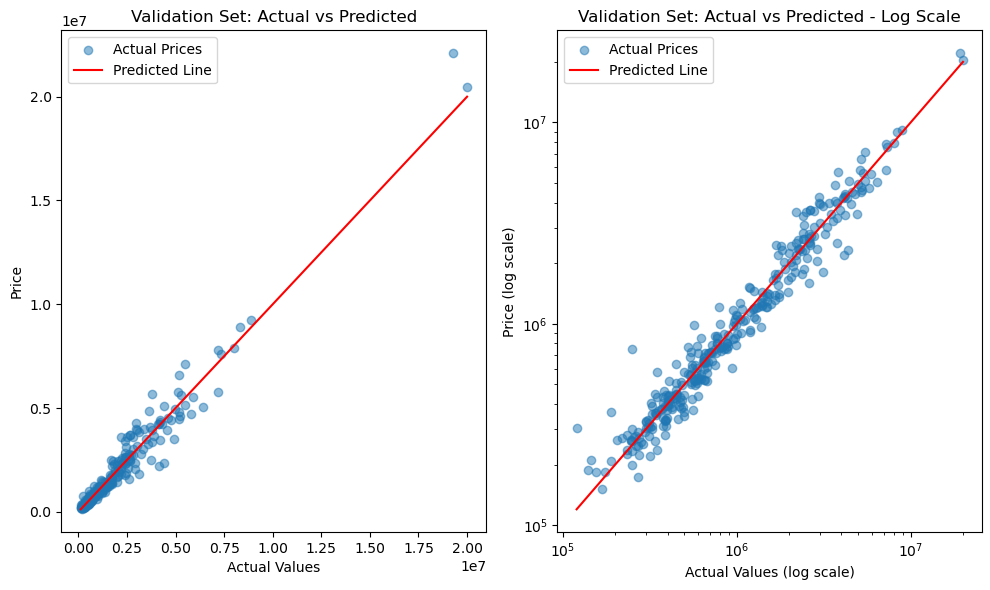
\includegraphics[width=\linewidth]{img/Poly_Validation_Plot.png}
        \caption{Đánh giá trên tập kiểm chứng}
        \label{fig:poly-linear-valid-plot}
    \end{subfigure}
    \caption{So sánh đánh giá mô hình hồi quy đa thức bậc 3 trên tập huấn luyện và kiểm chứng}
    \label{fig:poly-linear-eval-plot}
\end{figure}

\pagebreak

